% Quick start guide
\documentclass{beamer}

\usetheme{CambridgeUS}
\makeatletter
\setbeamertemplate{footline}{%
	\leavevmode%
	\hbox{%
		\begin{beamercolorbox}[wd=.3\paperwidth,ht=2.25ex,dp=1ex,center]{author in head/foot}%
			\usebeamerfont{author in head/foot}\insertshortauthor\expandafter\ifblank\expandafter{\beamer@shortinstitute}{}{~~(\insertshortinstitute)}
		\end{beamercolorbox}%
		\begin{beamercolorbox}[wd=.5\paperwidth,ht=2.25ex,dp=1ex,center]{title in head/foot}%
			\usebeamerfont{title in head/foot}\insertshorttitle
		\end{beamercolorbox}%
		\begin{beamercolorbox}[wd=.2\paperwidth,ht=2.25ex,dp=1ex,leftskip=2ex,rightskip=2ex,sep=0pt]{date in head/foot}%
			\hfill%
			\usebeamerfont{date in head/foot}%
			\insertshortdate{}%
			\hfill%
			\usebeamercolor[fg]{page number in head/foot}%
			\usebeamerfont{page number in head/foot}%
			\usebeamertemplate{page number in head/foot}%
	\end{beamercolorbox}}%
	\vskip0pt%
}
\makeatother

\centering\title{ Running a Carpentries Workshop without the Internet}
\date{September 5, 2023}

\author{JSS \inst{1} \and FT \inst{1} \and CS \inst{2} \\
	\and AD \inst{3} \and EPW \inst{4} \and SF \inst{5}}

\begin{document}
	\begin{frame}
		\begin{alertblock}
			
			Running a Carpentries Workshop without the Internet
		\end{alertblock}
		\begin{columns}
			\begin{column}{.4\textwidth}
				\centering
				\includegraphics[width=.6\columnwidth]{logos/carpentriesoffline_schemaidea.png} \\
				When the Internet is broken
				
			\end{column}
			\begin{column}{.4\textwidth}
				\centering
				\includegraphics[width=.4\columnwidth]{logos/OFFLINE_long.png}
				CarpentriesOffline offers three solutions
			\end{column}
			\end {columns}
			\begin{columns}
				\begin{column}{.33\textwidth}
					\centering
					\includegraphics[width=\columnwidth]{logos/CarpentriesOfflinePhoto.png}
					A Raspberry Pi
					
				\end{column}
				\begin{column}{.33\textwidth}
					\centering
					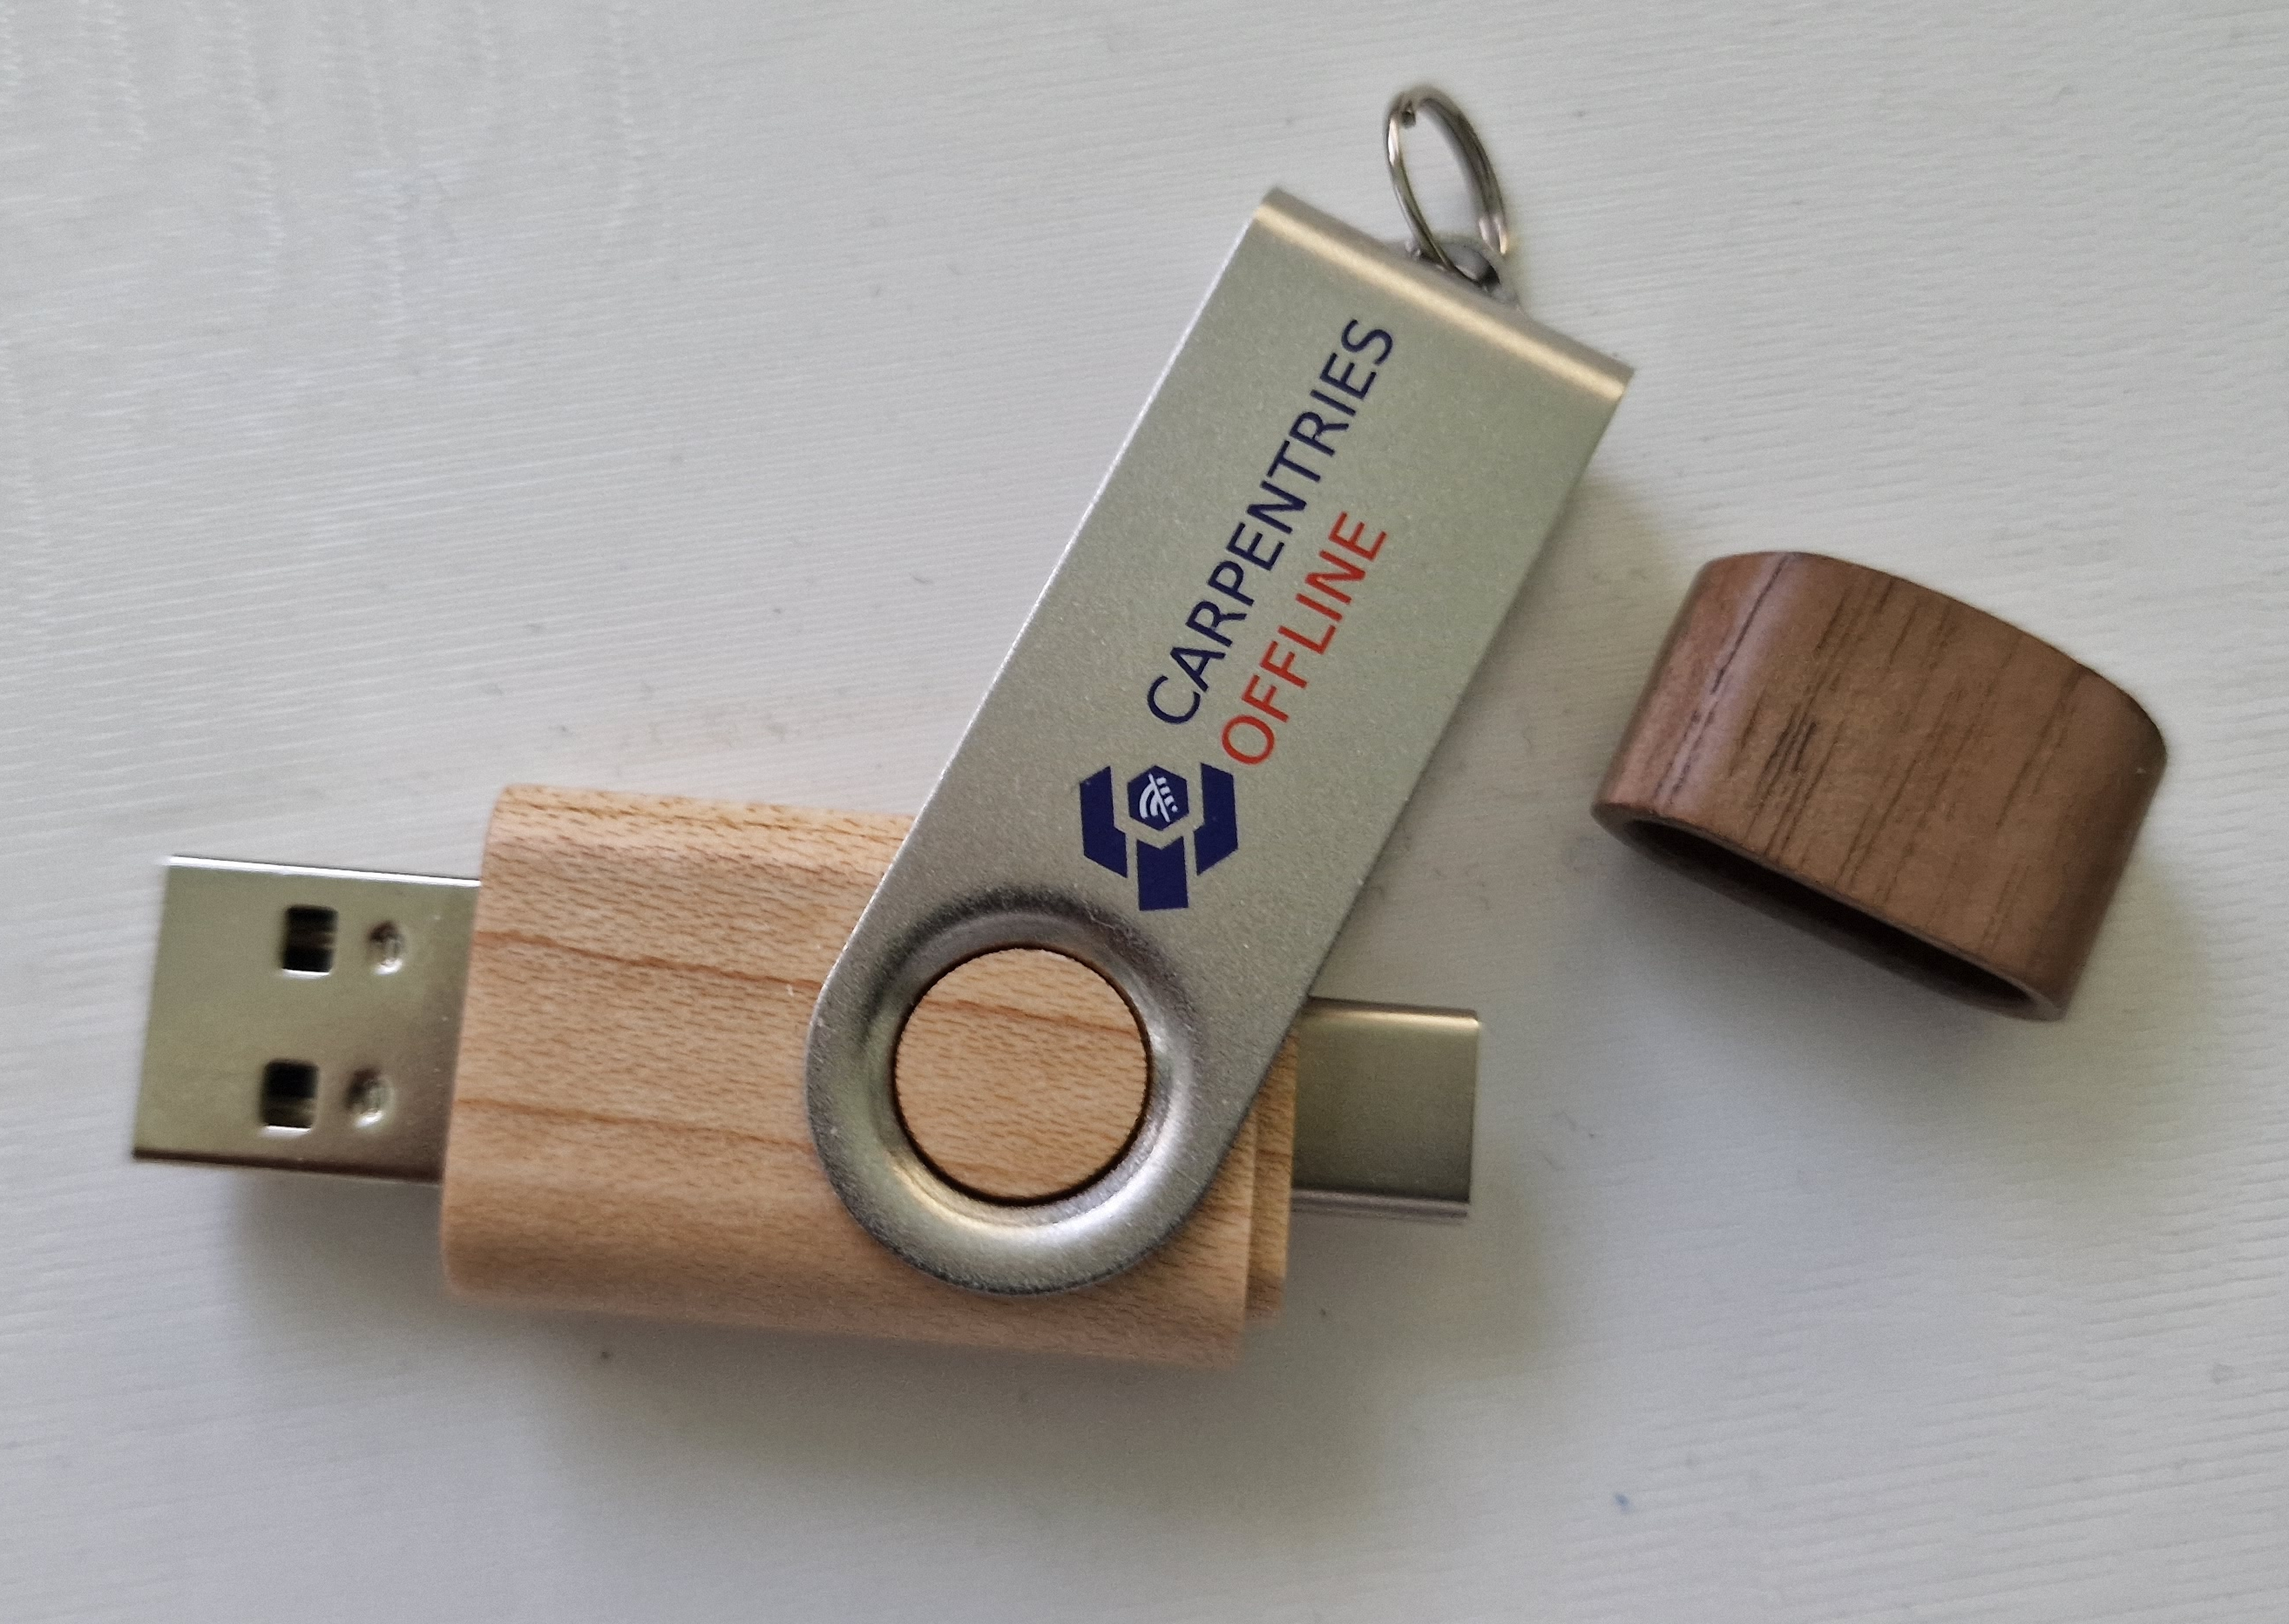
\includegraphics[width=\columnwidth]{logos/FlashDrive.png}
					A FlashDrive
					
				\end{column}
				\begin{column}{.33\textwidth}
					\centering
					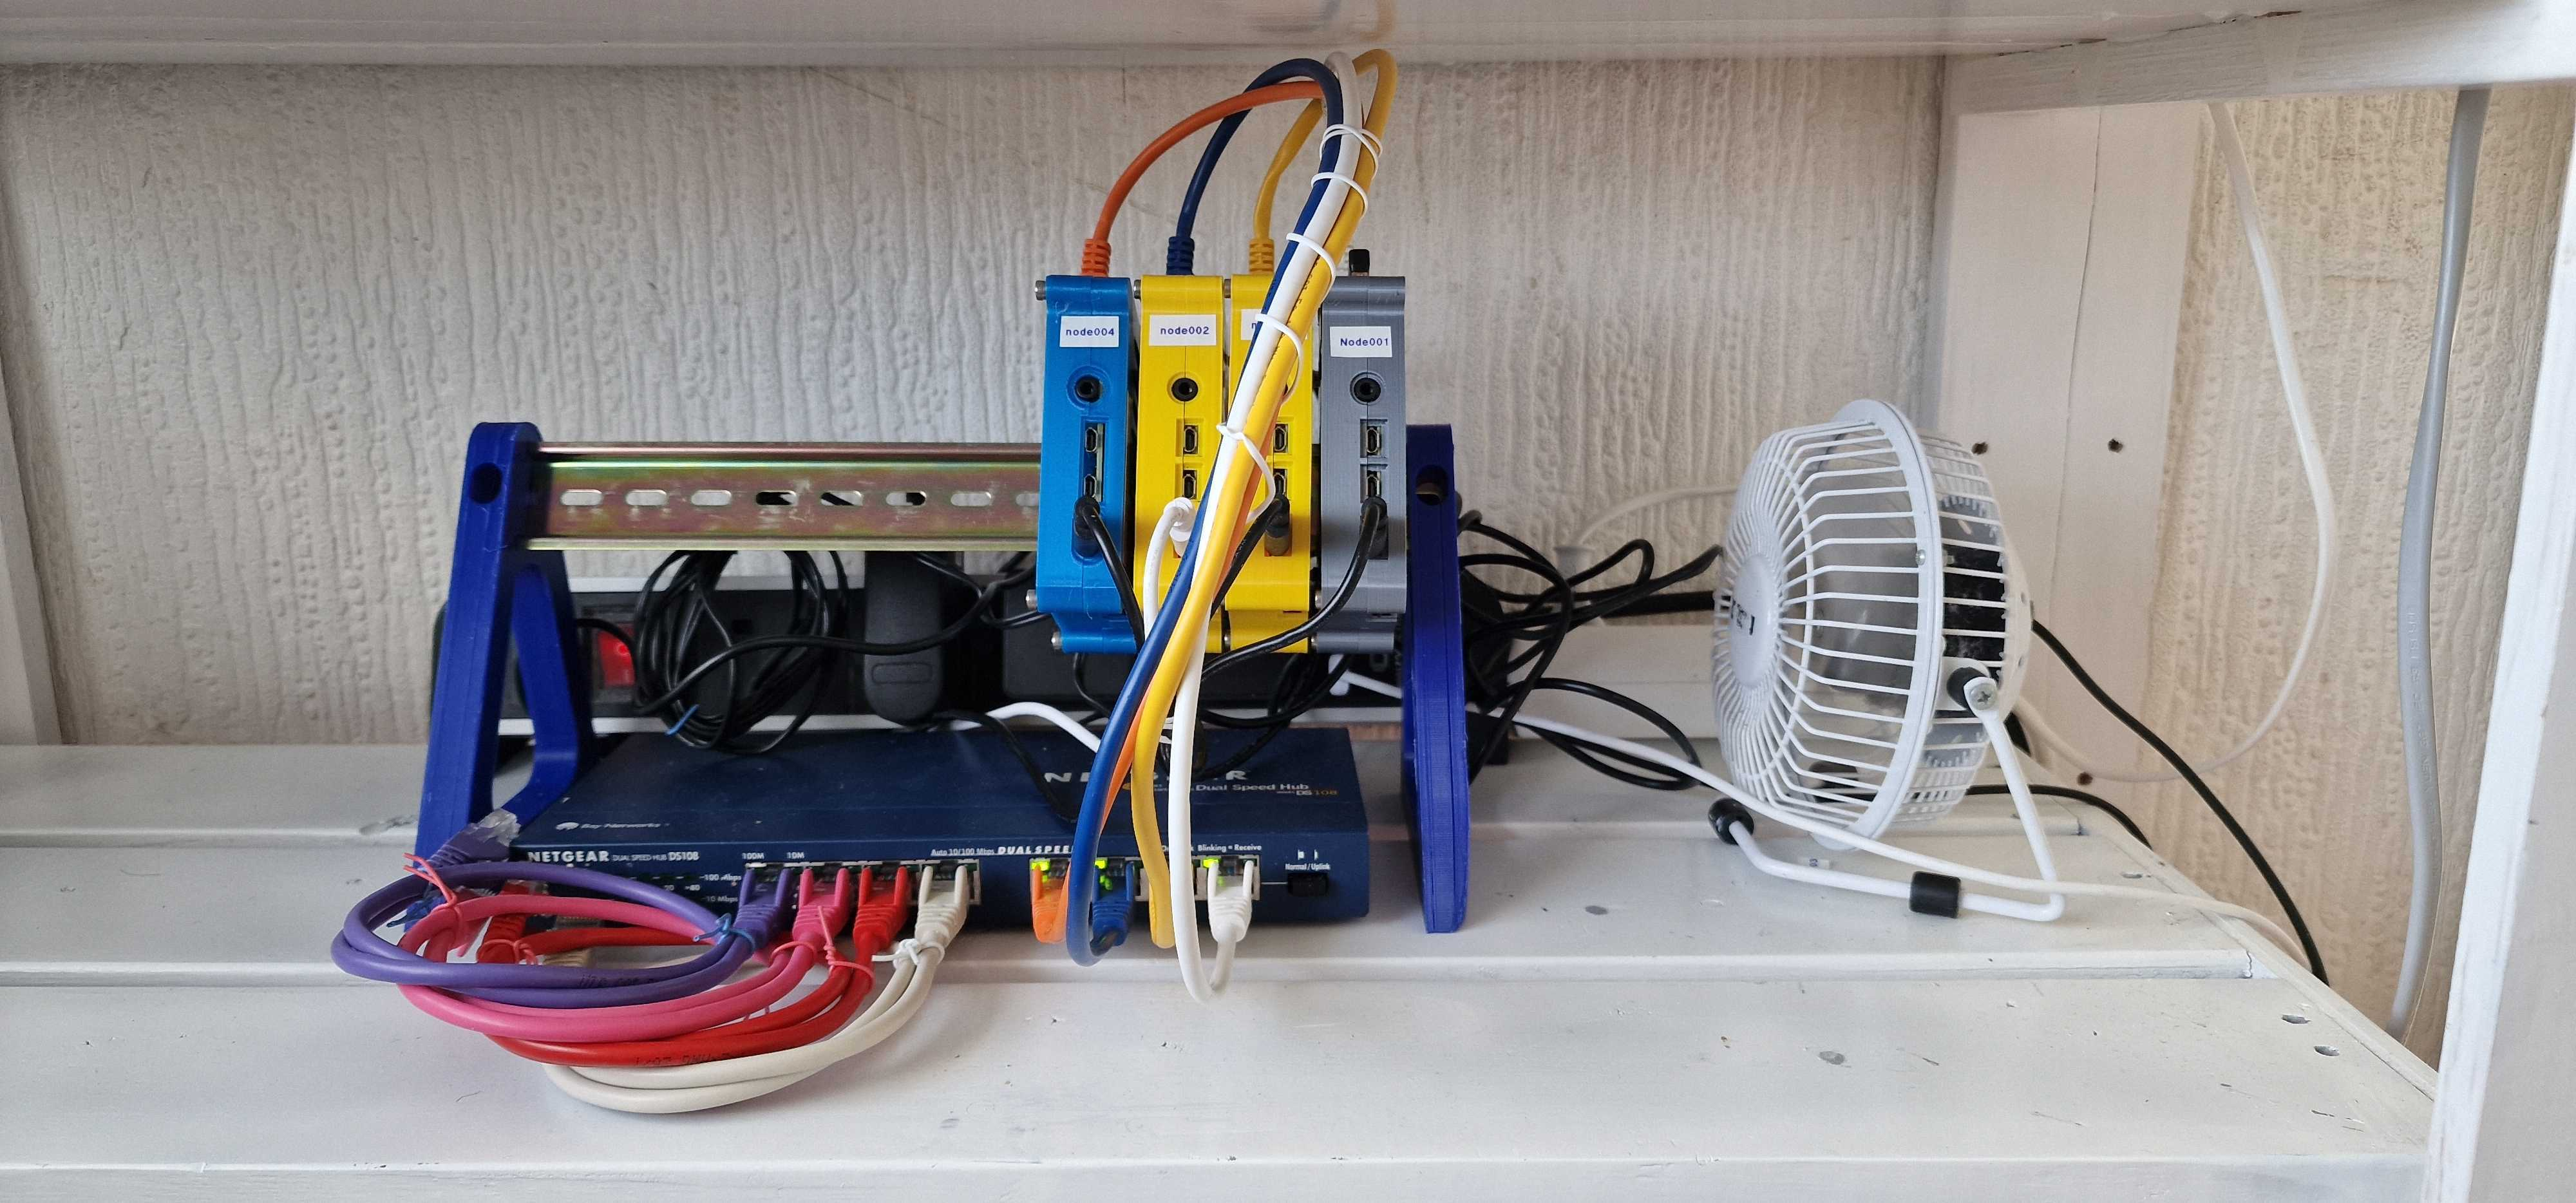
\includegraphics[width=\columnwidth]{logos/mini-HPC-proto1.png}
					A mini HPC
					
				\end{column}
			\end{columns}
			
			
		\end{frame}
	\end{document}
f